\chapter{Полученнные результаты}\label{chap1}

%%%%%%%%%%%%%%%%%%%%%%%%%%%%%%%%%%%%%%%%%%%%%%%%%%%%%%%%%%%%%%%%%%%%%%%%%%%%%%%%
\section{Обзор библиотеки gym}\label{1sec:optimal-control}
%%%%%%%%%%%%%%%%%%%%%%%%%%%%%%%%%%%%%%%%%%%%%%%%%%%%%%%%%%%%%%%%%%%%%%%%%%%%%%%%

Для решения исходной задачи используется библиотека gym, в которой имеется ее реализация. Библиотека gym -- это open-source набор инструментов для разработки и сравнения алгоритмов обучения с подкреплением. Данная библиотека не делает никаких предположений о структуре агента и совместима с любой библиотекой численных вычислений, такой как TensorFlow или Pytorch. В ней собраны и реализованы классические задачи оптимального управления и несколько игровых задач. 

Сама библиотека симулирует среду. Таким образом агент может подавать в среду действие, а на выходе получать награду и состояние среды. Самый простой способ запустить ее вызов на 1000 шагов с выбором случайного действия из набора всех возможных действий представлен ниже. 

\begin{minted}[mathescape, linenos]{python}
import gym 
env = gym.make('Pendulum-v0')
env.reset() 
for i in range(1000): 
    env.render() 
    env.step(env.action_space.sample()) # take a random action 
env.close()
\end{minted}

Таким образом \mintinline{python}{env} -- это непосредственно среда. Для сброса ее в начальное состояние используется команда \mintinline{python}{env.reset()}. \mintinline{python}{env.redner()} рисует картинку полученного состояния текущей среды. Пример можно найти на рисунке ~\ref{fig:cart-pole}. Множество всех доступных действий можно найти с помощью команды \mintinline{python}{env.action_space}. Чтобы совершить действие нужно вызвать команду \mintinline{python}{env.step(action)} и передать в него необходимое действие (\mintinline{python}{action}). В ответ на это среда вернет четыре параметра \mintinline{python}{(observation, reward, done, info)}. Которые обозначают следующее:
\begin{itemize}
	\item observation -- состояние среды, наблюдаемое после совершенного действия.
	\item reward -- полученная награда от совершенного действия.
	\item done -- завершена ли текущая задача.
	\item info -- вспомогательная информация, используемая для отладки. 
\end{itemize}
 \newpage


\begin{figure}[h]
	\centering
	\includegraphics[scale=1.2]{download.png}
	\caption {Пример обратного маятника}
	\label{fig:cart-pole}
\end{figure}

%%%%%%%%%%%%%%%%%%%%%%%%%%%%%%%%%%%%%%%%%%%%%%%%%%%%%%%%%%%%%%%%%%%%%%%%%%%%%%%%
\section{Формулировка поставленной задачи оптимального управления и ее решением методом q-обучения}\label{1sec:optimal-control}
%%%%%%%%%%%%%%%%%%%%%%%%%%%%%%%%%%%%%%%%%%%%%%%%%%%%%%%%%%%%%%%%%%%%%%%%%%%%%%%%

В данной работе рассмотрим задачу оптимального управления — маятник. Общая формулировка задана уравнением (~\ref{eq:pend}.) 

Для решения задачи использовалась библитека gym, описанная выше. В ней маятник выглядит как представлен на рисунке ~\ref{fig:pend}. 

\begin{figure}[h]
	\centering
	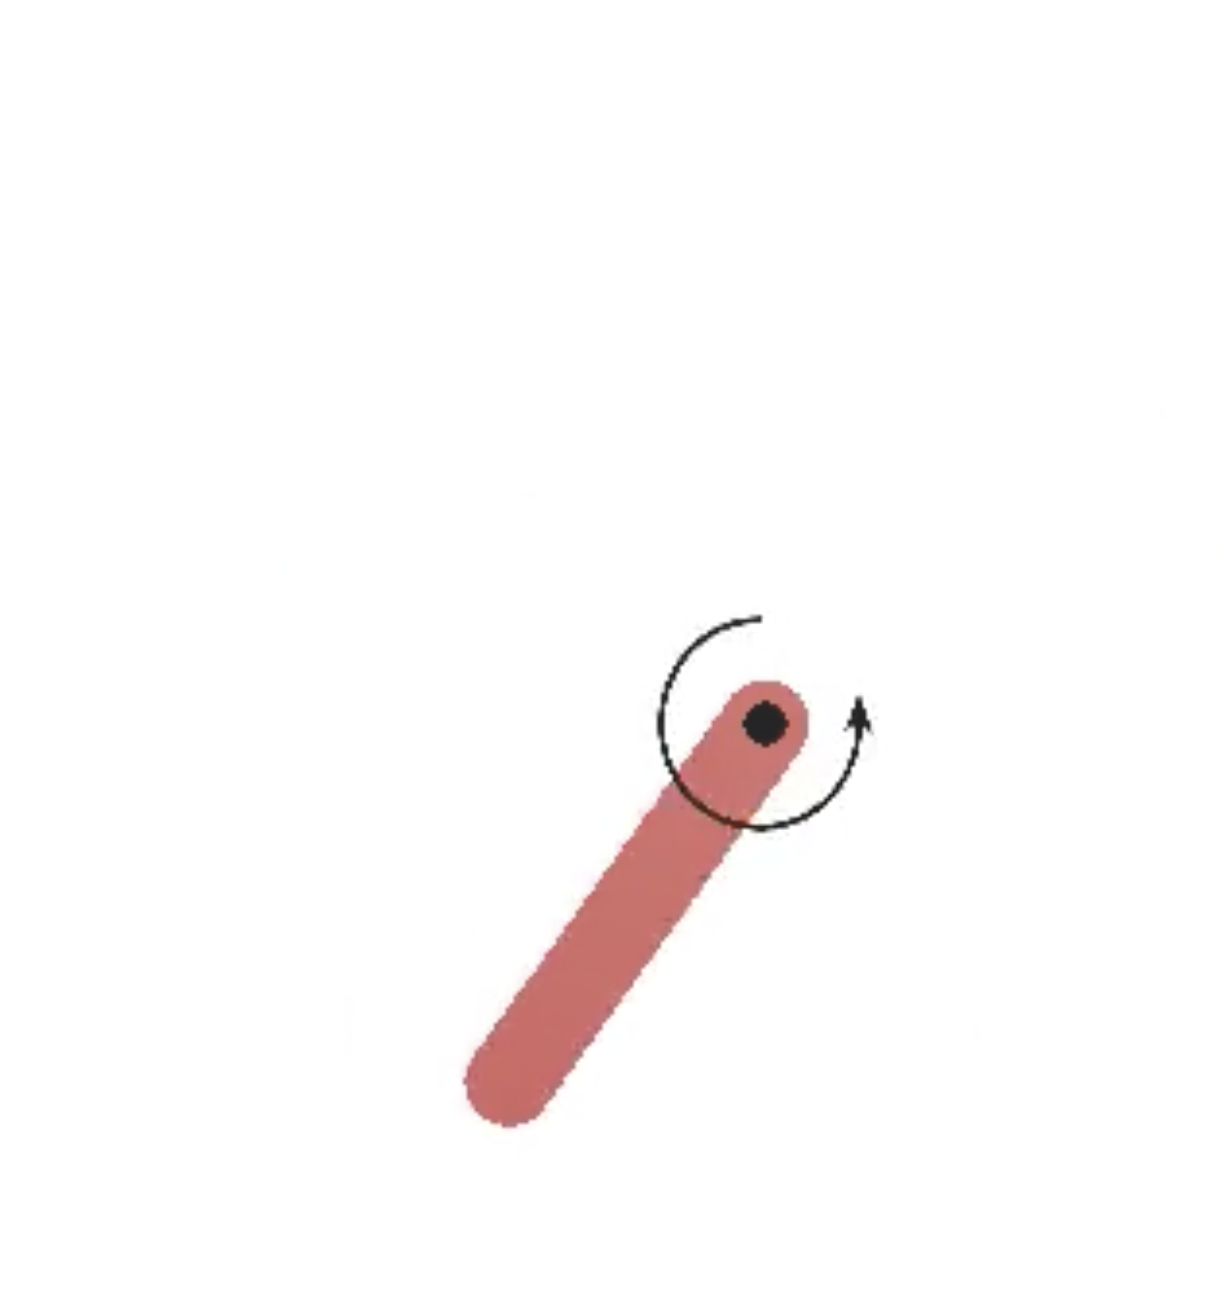
\includegraphics[scale=0.2]{pend.png}
	\caption {Маятник в библиотеке gym}
	\label{fig:pend}
\end{figure}


В рамках данной задачи есть одна переменная $\phi$ -- угол отклонения маятника от вертикальной оси. На переменную накладываются следующие ограничения:
\begin{equation}
	\begin{aligned}
		\phi_{min} \leq \phi \leq \phi_{max}.
	\end{aligned}
\end{equation}

Визуальное представление того, как угол отсчитывается от оси находится на рисунке ~\ref{fig:pend2}.

\begin{figure}[h]
	\centering
	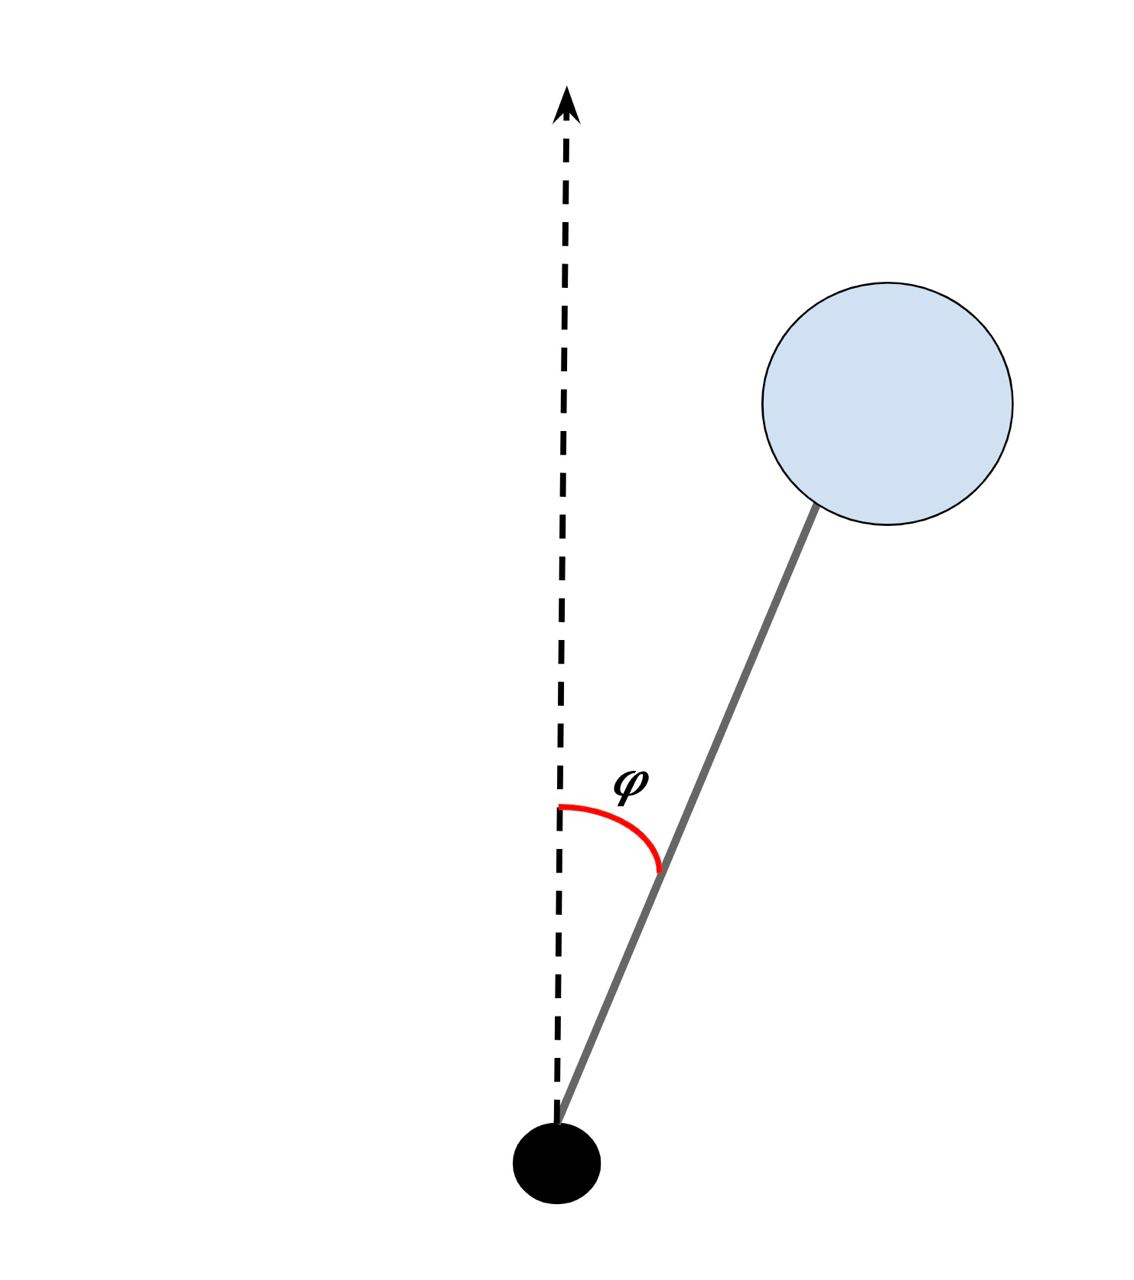
\includegraphics[scale=0.3]{pend2.jpg}
	\caption {Маятник}
	\label{fig:pend2}
\end{figure}

В нашем случае вводятся следующие ограничения:
$\phi_{min} = -180^\circ$,  $\phi_{max} = 180^\circ$. 
Кроме того рассматривается непрерывное управление (действия): $u = [-2, 2]$, то есть либо толкнуть маятник вправо, либо влево с максимальным модулем силы $2$.

За каждое действие дается награда $r \in (-\infty, \infty)$. Цель задачи -- при 200 запусках сессий  привести маятник в вертикальное положение и сохранять его в таком положении. 

Для решения задачи использовался алгоритм q-обучения в рамках которого функция $q(s, a)$ считалась с помощью архитектуры нейронной сети представленной на рисунке ~\ref{fig:q-nn}.

\begin{figure}[h]
	\centering
	\includegraphics[scale=0.39]{nn1.png}
	\caption {Архитектура сети для подсчета $q(s, a)$}
	\label{fig:q-nn}
\end{figure}

\newpage

В рамках решения задачи использовалась эпсилон-жадная политика. То есть на каждой итерации с вероятностью в $\epsilon$ вместо лучшего действия выбиралось случайное. На каждой эпохе обучения мы запускам 10 сессий и считаем среднюю полученную награду. График обучения представлен на рисунке ~\ref{fig:rews}.

\newpage

\begin{figure}[h]
	\centering
	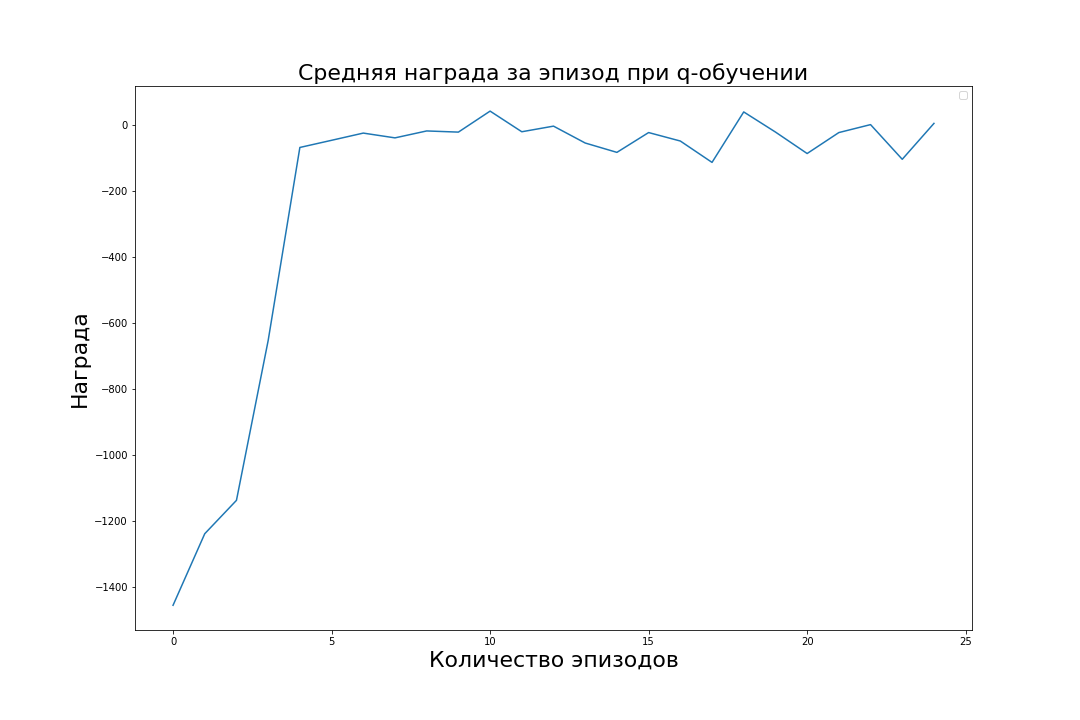
\includegraphics[scale=0.5]{rews.png}
	\caption {График q-обучения}
	\label{fig:rews}
\end{figure}



%%%%%%%%%%%%%%%%%%%%%%%%%%%%%%%%%%%%%%%%%%%%%%%%%%%%%%%%%%%%%%%%%%%%%%%%%%%%%%%%
\section{Решение задачи методом MPC }\label{1sec:optimal-control}
%%%%%%%%%%%%%%%%%%%%%%%%%%%%%%%%%%%%%%%%%%%%%%%%%%%%%%%%%%%%%%%%%%%%%%%%%%%%%%%%

%%%%%%%%%%%%%%%%%%%%%%%%%%%%%%%%%%%%%%%%%%%%%%%%%%%%%%%%%%%%%%%%%%%%%%%%%%%%%%%%
\subsection{Решение задачи методом MPC с помощью робастного метода кросс-энтропии }\label{1sec:optimal-control}
%%%%%%%%%%%%%%%%%%%%%%%%%%%%%%%%%%%%%%%%%%%%%%%%%%%%%%%%%%%%%%%%%%%%%%%%%%%%%%%%

В рамках данной задачи согласно схеме из рисунка ~\ref{fig:mpc-m} мы обучали модель среды и параллельно запускали и обучали метод MPC с помощью робастного метода кросс энтропии. Горизонт планирования для МРС  составлял $T=200$, так как эпизод рассчитан на 200 действий. В результате обучения модель научилась довольно точно предсказывать следующее состояние среды. График ошибки состояния среды представлен на рисунке ~\ref{fig:obs}. Кроме того модель среды научилась довольно точно предсказывать награду. График абсолютной ошибки предсказанной награды представлен на рисунке ~\ref{fig:rew-err}. Ошибка считалась с помощью средней абсолютной ошибки:
\begin{equation}
	err = \dfrac{\sum\limits_{i=0}^N |x_i - y_i|}{N},
	\label{eq:err}
\end{equation}
где $x_i$ -- полученное измерение, $y_i$ -- истинное значение.
\begin{figure}[!htb]
	\centering
	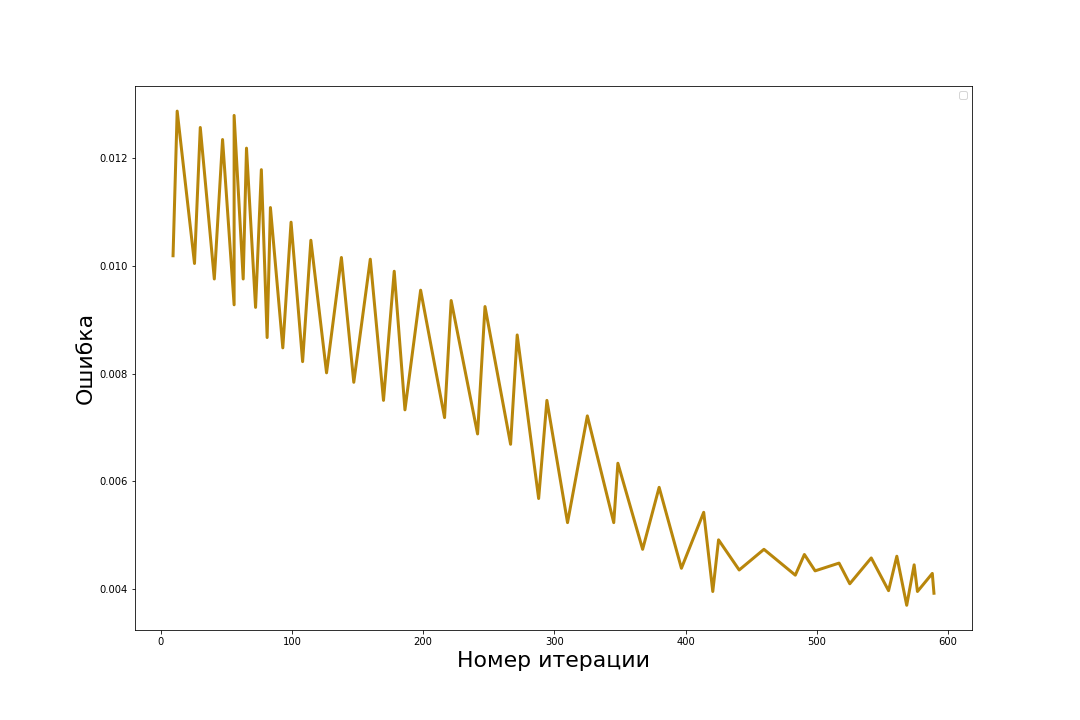
\includegraphics[scale=0.44]{obs.png}
	\caption {График абсолютной ошибки состояния среды}
	\label{fig:obs}
\end{figure}



\begin{figure}[!htb]
	\centering
	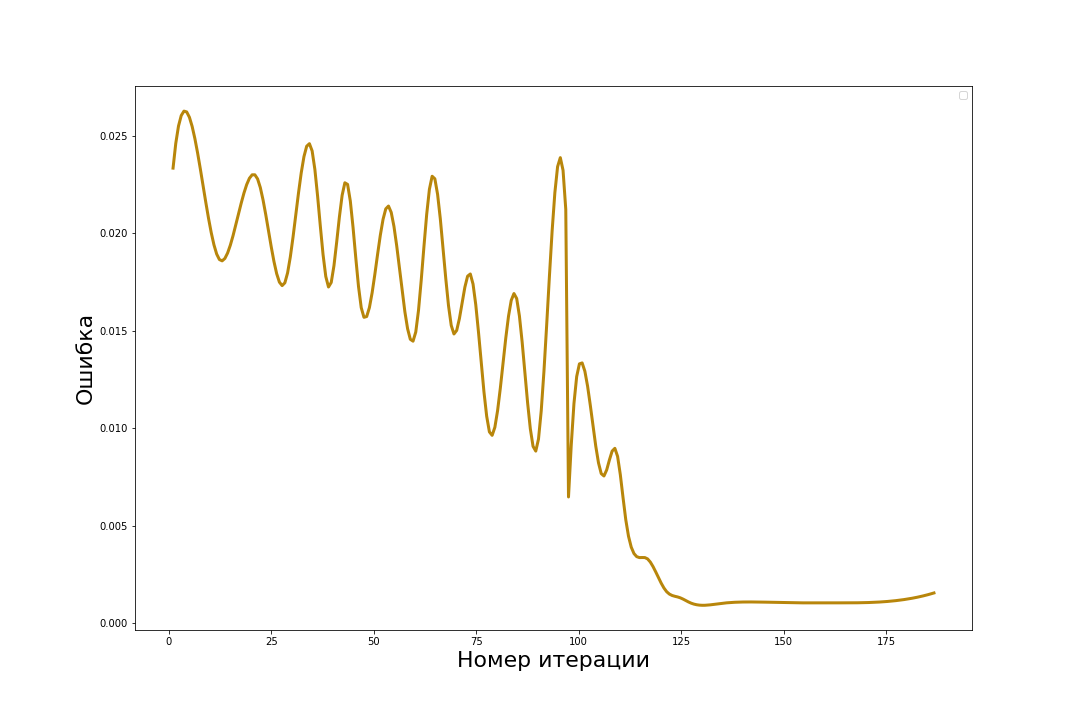
\includegraphics[scale=0.44]{rew_err.png}
	\caption {График абсолютной ошибки награды}
	\label{fig:rew-err}
\end{figure}

\newpage
По мере обучения ошибка, используемая нейронной сетью для модели среды падала. График представлен на рисунке ~\ref{fig:loss}. Таким образом модель среды все больше становится похожа непосредственно на среду. 


\begin{figure}[!htb]
	\centering
	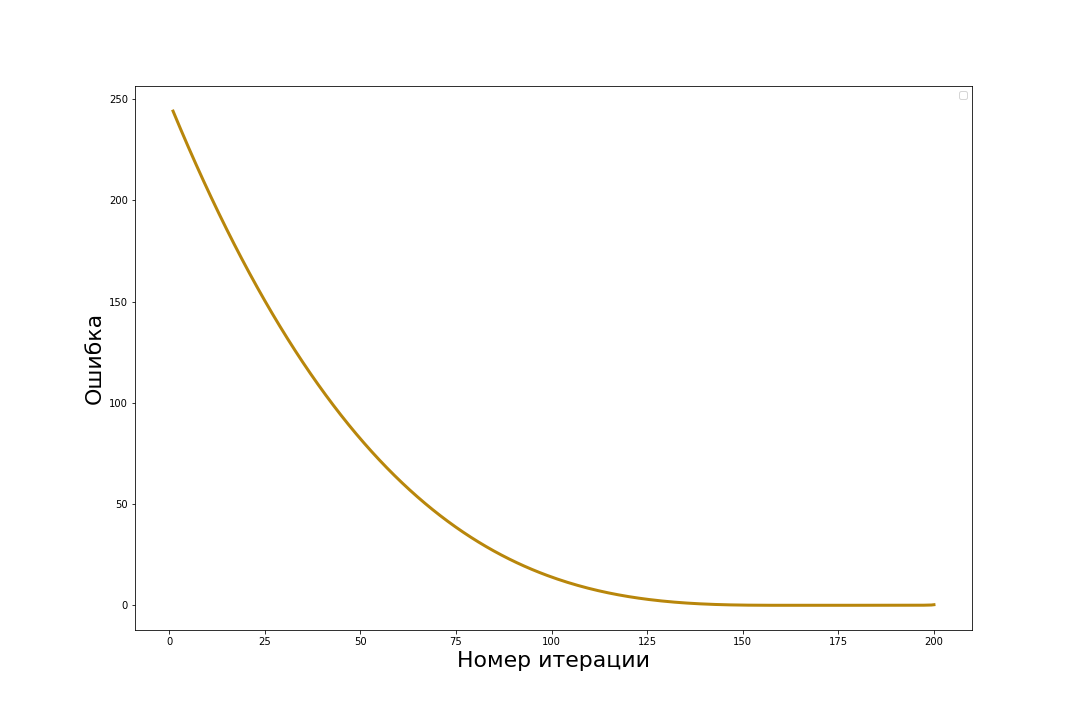
\includegraphics[scale=0.5]{loss.png}
	\caption {График ошибки модели среды}
	\label{fig:loss}
\end{figure}

Средняя реальная награда за эпизод (200 действий), которую получает наш агент за каждое действие растет по мере обучения. График чего представлен на рисунке ~\ref{fig:rew}.  \newpage


\begin{figure}[!htb]
	\centering
	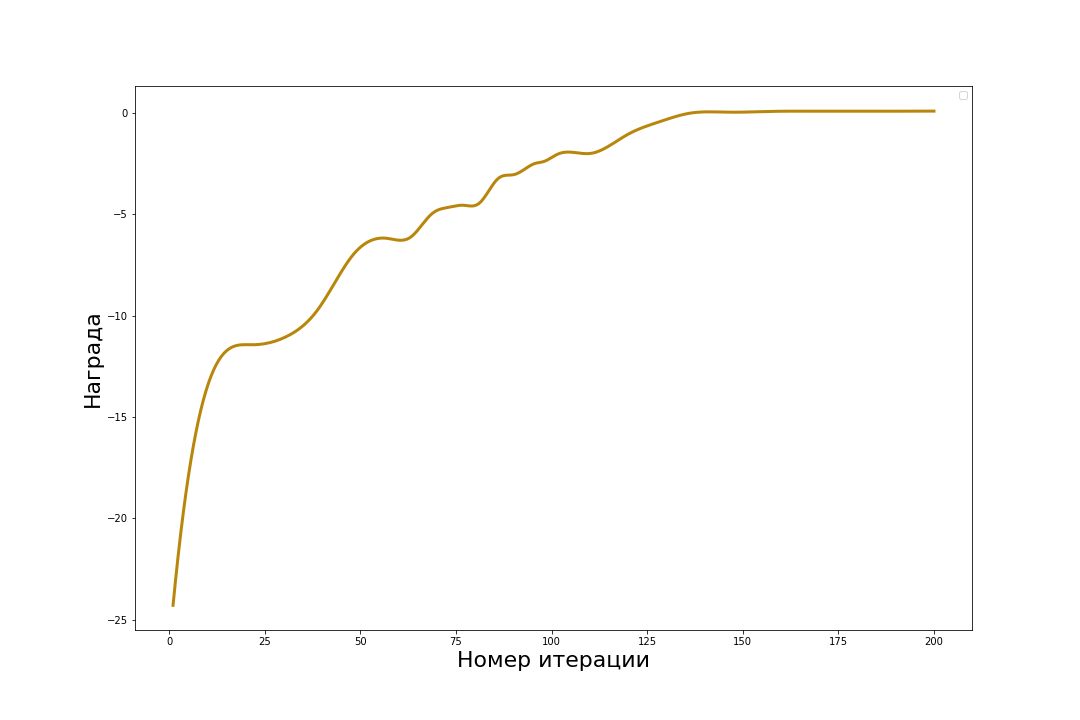
\includegraphics[scale=0.5]{rew.png}
	\caption {Абсолютная награда}
	\label{fig:rew}
\end{figure}



%%%%%%%%%%%%%%%%%%%%%%%%%%%%%%%%%%%%%%%%%%%%%%%%%%%%%%%%%%%%%%%%%%%%%%%%%%%%%%%%
\subsection{Решение задачи методом MPC на предобученной модели среды}\label{1sec:optimal-control}
%%%%%%%%%%%%%%%%%%%%%%%%%%%%%%%%%%%%%%%%%%%%%%%%%%%%%%%%%%%%%%%%%%%%%%%%%%%%%%%%

Теперь сначала потренируем модель среды, генерируя действия случайно и посмотрим даст ли нам это улучшений. Сначала посмотрим на полученные результаты. Они приведены на рисунках ~\ref{fig:pretr-err} и ~\ref{fig:pretr-reward}. Ошибка считается по формуле ~\ref{eq:err}. 

Видно, что данный метод работает хуже, чем исходный. Из-за предобучения на политике, которая генерирует случайные действия и состояния, наша модель среды хуже предсказывает следующее состояние среды и хуже предсказывает получаемую награду. Это можно легко объяснить тем, что в данном случае наш маятник просто качается из случайного положения в случайное и награда все время становится очень маленькой. Поэтому когда позже мы начинаем применять политику, которую выдает MPC, состояния мало коррелируют с теми, на которых обучалась модель. В результате чего получаются очень плохие предсказания. Поэтому в дальнейшем не будем предобучать модель среды на случайной политике, а будем обучать ее совместно с MPC.

\newpage


\begin{figure}[!htb]
	\centering
	\includegraphics[scale=0.44]{pretr_error.png}
	\caption {График ошибки состояния для предобученной модели. }
	\label{fig:pretr-err}
\end{figure}


\begin{figure}[!htb]
	\centering
	\includegraphics[scale=0.44]{pretr_reward.png}
	\caption {График ошибки награды для предобученной модели. }
	\label{fig:pretr-reward}
\end{figure}


%%%%%%%%%%%%%%%%%%%%%%%%%%%%%%%%%%%%%%%%%%%%%%%%%%%%%%%%%%%%%%%%%%%%%%%%%%%%%%%%
\subsection{Решение задачи методом MPC с реальной средой}\label{1sec:optimal-control}
%%%%%%%%%%%%%%%%%%%%%%%%%%%%%%%%%%%%%%%%%%%%%%%%%%%%%%%%%%%%%%%%%%%%%%%%%%%%%%%%

Попробуем посмотреть, насколько хороши наши результаты в сравнении с тем, если бы мы обучались непосредственно на взаимодействии со средой. Результаты получаемой награды для такого обучения представлены на рисунке ~\ref{fig:true-rew}. В результате награда также сходится к 0.


\begin{figure}[!h]
	\centering
	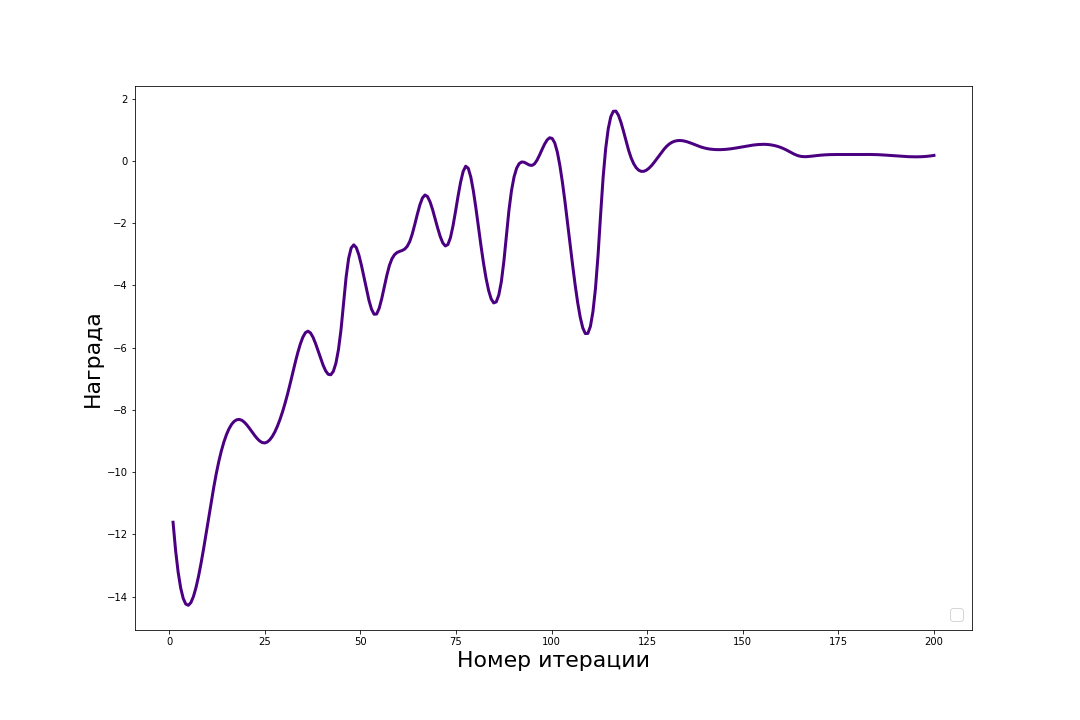
\includegraphics[scale=0.5]{true_reward.png}
	\caption {Награда в реальной среде}
	\label{fig:true-rew}
\end{figure}

Сравним с наградой, которую получаем на претренированной модели, которая была представлена на рисунке ~\ref{fig:rew}. График представлен на рисунке ~\ref{fig:comp-rew}. Видно, что награда, полученная непосредственно на взаимодействии со средой быстрее сходится к 0. Это объяснимо тем, что модель не сразу полностью повторяет среду, а с каждой итерацией все больше приближается к ней. Поэтому и награда растет не так быстро. Однако в итоге и в одном, и во втором случае награда становится сравнимой. Таким образом подход с обучением модели среды не ухудшает политику выбора действия агента, а доход в результате остается сравнимым. То есть model-based алгоритм не ухудшает результаты в сравнении с model-free алгоритмом. \newpage


\begin{figure}[!h]
	\centering
	\includegraphics[scale=0.5]{comp_reward.png}
	\caption {График сравнение наград настоящей среды и модели среды}
	\label{fig:comp-rew}
\end{figure}


%%%%%%%%%%%%%%%%%%%%%%%%%%%%%%%%%%%%%%%%%%%%%%%%%%%%%%%%%%%%%%%%%%%%%%%%%%%%%%%%
\subsection{Сравнение двух методов обучения MPC для решения задачи  }\label{1sec:optimal-control}
%%%%%%%%%%%%%%%%%%%%%%%%%%%%%%%%%%%%%%%%%%%%%%%%%%%%%%%%%%%%%%%%%%%%%%%%%%%%%%%%

Теперь будем обучать MPC с помощью второго алгоритма, описанного в главе 3 -- эволюционной стратегии адаптации ковариационной матрицы. Полученные результаты в сравнении с результатами обучения методом робастной кросс-энтропии (рисунки ~\ref{fig:obs}, ~\ref{fig:rew-err}, ~\ref{fig:rew}) представлены на рисунках ~\ref{fig:mca-obs}, ~\ref{fig:mca-rew-err}, ~\ref{fig:mca-rew}. Ошибка считается по формуле (~\ref{eq:err}). На рисунках видно, что новый алгоритм дает более быструю сходимость к получению награды. Кроме того быстрее обучает модель среды, а именно быстрее сходится к меньшей ошибке состояния среды. Таким образом он является предпочтительным для решения данной задач с помощью MPC. \newpage

\begin{figure}[!h]
	\centering
	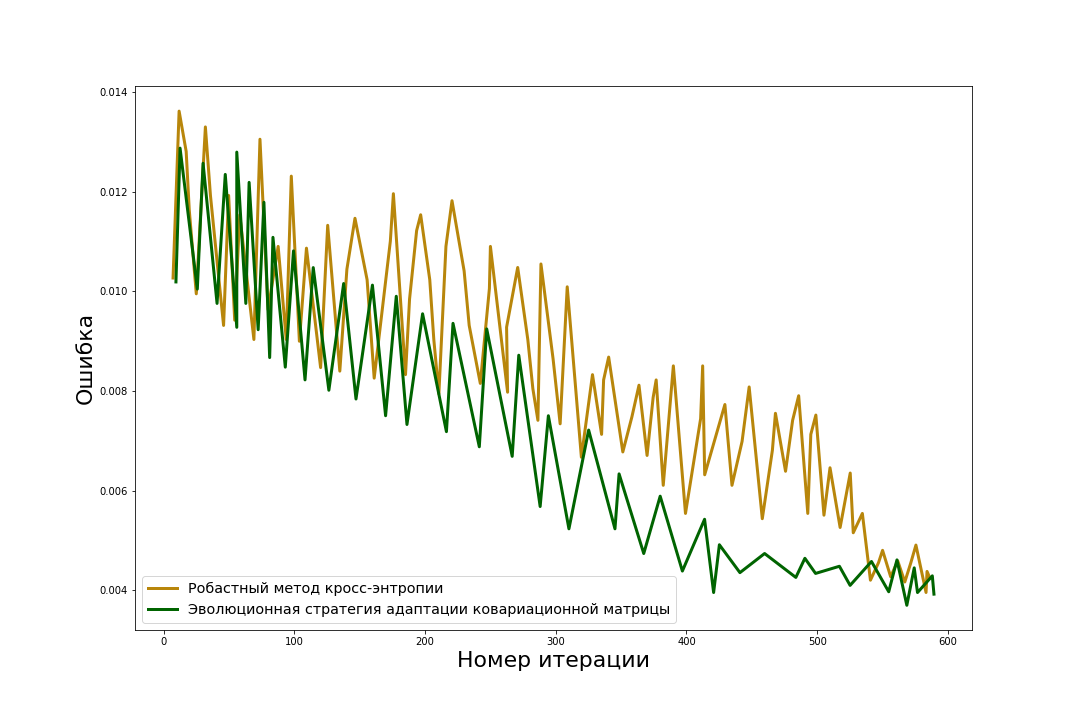
\includegraphics[scale=0.44]{mca_obs.png}
	\caption {График сравнение ошибки состояния}
	\label{fig:mca-obs}
\end{figure}



\begin{figure}[!h]
	\centering
	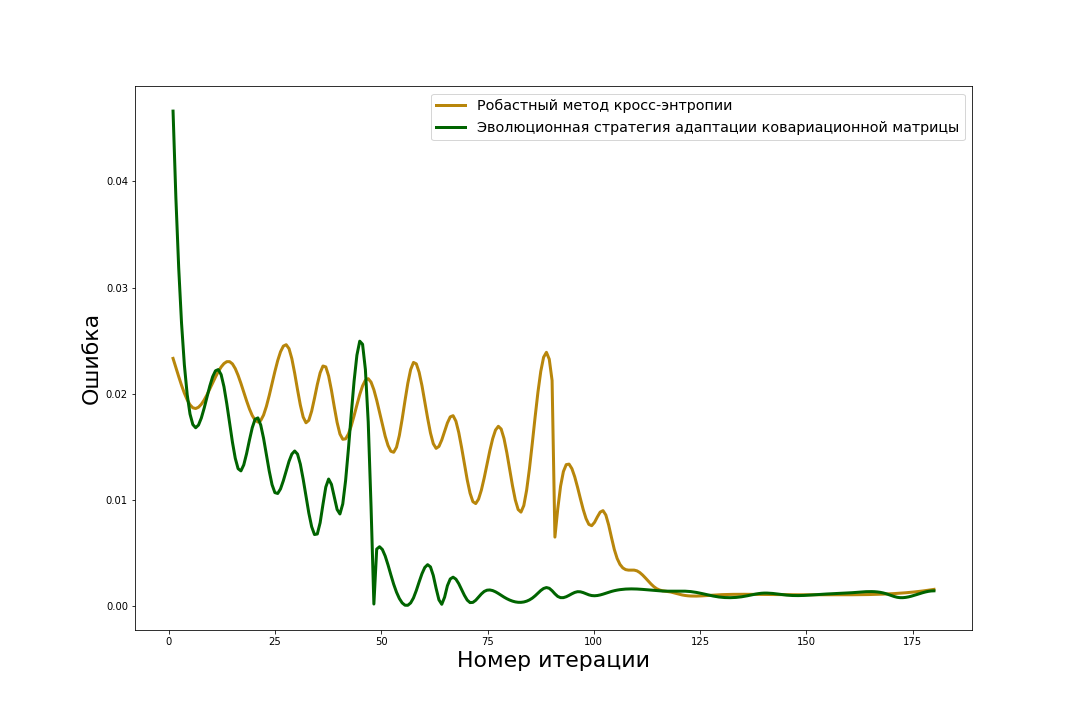
\includegraphics[scale=0.44]{mca_rew_err.png}
	\caption {График сравнение ошибки награды}
	\label{fig:mca-rew-err}
\end{figure}


\begin{figure}[!h]
	\centering
	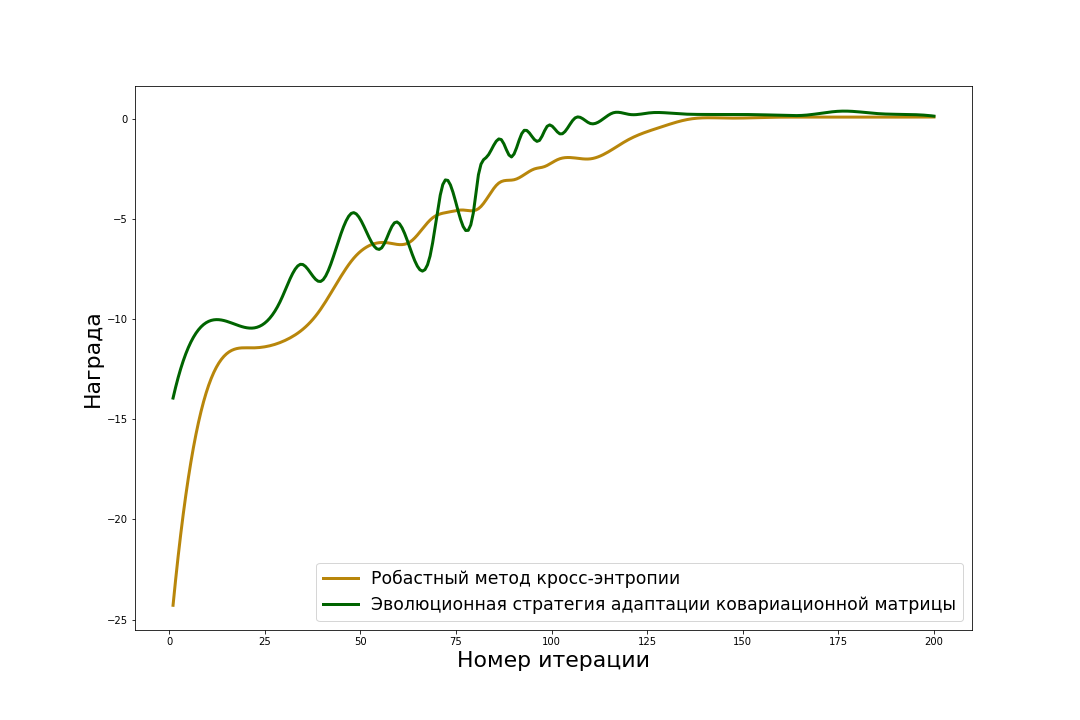
\includegraphics[scale=0.5]{mca_reward.png}
	\caption {График сравнение наград}
	\label{fig:mca-rew}
\end{figure}

 
 %%%%%%%%%%%%%%%%%%%%%%%%%%%%%%%%%%%%%%%%%%%%%%%%%%%%%%%%%%%%%%%%%%%%%%%%%%%%%%%%
 \section{Сравнение решения методом MPC  и q-обучением}\label{1sec:optimal-control}
 %%%%%%%%%%%%%%%%%%%%%%%%%%%%%%%%%%%%%%%%%%%%%%%%%%%%%%%%%%%%%%%%%%%%%%%%%%%%%%%%

Возьмем МРС, обученный на модели среды с помощью эволюционной стратегии адаптации ковариационной матрицы и используя его стратегию сыграем 1000 сессий маятника и сравним полученные результаты с 1000 сессиями работы маятника, в которых используется политика выбора действия, полученная в результате q-обучения. Результаты среднего полученной награды, ее среднеквадратичного отклонения, минимума и максимума приведены в таблице ~\ref{tab:comp}. Как видно из нее в среднем МРС работает лучше, к тому же разброс значений (стандартное отклонение) у него меньше. Кроме того экстремальные значения (минимум и максимум) у МРС ближе к среднему. Таким образом решение с помощью МРС выдает лучшие результаты, чем q-обучение. Разница между ними не так велика, однако МРС еще и не нарушает исходные ограничения. Таким образом лучше решает поставленную задачу.  
 

\begin{minipage}{\linewidth}
	\begin{center}
	\begin{tabular}{ >{\centering\arraybackslash}m{1.5in} *4{>{\centering\arraybackslash}m{.75in}}}
		\toprule[1.5pt]
		 \bf Метод  & \bf Mean & \bf Std & \bf Min & \bf Max\\
		 \midrule
		MPC    & 0.5      &  3     & -7    & 2\\
		\midrule
		Q-обучение    & -4      &  15     & -30    & 5\\
		\bottomrule[1.25pt]
		\end{tabular}\par
		\bigskip
		\captionsetup{justification=centering}
		\captionof{table}{Сравнение q-обучения и MPC} 
		\label{tab:comp}
		\end{center} 
\end{minipage}



%%%%%%%%%%%%%%%%%%%%%%%%%%%%%%%%%%%%%%%%%%%%%%%%%%%%%%%%%%%%%%%%%%%%%%%%%%%%%%%%
\section{Выводы}\label{1sec:optimal-control}
%%%%%%%%%%%%%%%%%%%%%%%%%%%%%%%%%%%%%%%%%%%%%%%%%%%%%%%%%%%%%%%%%%%%%%%%%%%%%%%%

В данной главе были представлены результаты экспериментов, результате которых была решена поставленная задача методом q-обучения. Кроме того было получено, что данный метод работает несколько хуже, чем MPC. Также исходная задача была решена методом MPC с помощью алгоритма робастной кросс-энтропии и эволюционной стратегии адаптации ковариационной матрицы. Было получено, что второй алгоритм дает более быструю сходимость и является предпочтительным. Также было найдено, что обучение на модели среды работает несколько хуже, чем на реальной среде. Однако в  результате и один, и второй способ сходятся к одинаковой награде. Кроме того было показано, что не имеет смысла предобучать модель на политике, которая выбирает случайное действие.
